\documentclass[a4paper,indent]{paper}
\usepackage{tikz}
\usepackage{microtype}
\usepackage{inputenc}
\usepackage{rotating}
\usepackage{fullpage}
\usepackage{caption}
\usepackage{tikz}
\usepackage{tikz-timing}
\usepackage{mdframed}
\usepackage{fourier} % for /danger
\usepackage{amsmath}
\usepackage{acronym}
\usepackage[hidelinks]{hyperref}

\usetikzlibrary{arrows, shapes.gates.logic.US, calc}
%\usetikzlibrary{external} % doesn't work with tikz timing diagrams
%\tikzexternalize % activate!

\title{Auger Radio Digitizer}
\subtitle{Software and Hardware Interfaces}
\author{%
  Sjoerd T. Timmer (s.timmer@astro.ru.nl)\\
  Roel Jordans (r.jordans@astro.ru.nl)}
\date{}


\acrodef{RD}[RD]{Radio Digitizer}
\acrodef{UUB}[UUB]{Universal Upgrade Board}
\acrodef{SPI}[SPI]{Serial Peripheral Interface}
\acrodef{ADC}[ADC]{analog-to-digital converter}
\acrodef{FPGA}[FPGA]{field programmable gate array}
\acrodef{DDR}[DDR]{double data rate}
\acrodef{GPIO}[GPIO]{general-purpose IO}
\acrodef{LNA}[LNA]{low-noise amplifier}
\acrodef{PGA}[PGA]{programmable-gain amplifier}
\acrodef{MSB}[MSB]{most-significant bit}
\acrodef{I2C}[$\text{I}^2\text{C}$]{}
\acused{I2C}
%\newmdenv[linecolor=orange,backgroundcolor=orange!10]{warning}

\newenvironment{warning}
{\par\begin{mdframed}[linewidth=2pt,linecolor=orange,backgroundcolor=orange!10]%
    \begin{list}{}{\leftmargin=0mm}\item[\bf\danger{}~~Warning: ]}
  {\end{list}\end{mdframed}\par}

\newenvironment{deprecation}
{\par\begin{mdframed}[linewidth=1pt,linecolor=black,backgroundcolor=black!10]%
    \begin{list}{}{\leftmargin=0mm}\item[\bf\danger{}~~Old behaviour: ]}
  {\end{list}\end{mdframed}\par}



\begin{document}
\maketitle{}
\begin{abstract}
  This document describes the Auger \acf{RD} module and the external interface to the \acs{UUB} board.
  For an overview of the internal architecture refer to the RD Software Developer's Guide.
  \acresetall
\end{abstract}

\begin{mdframed}[linewidth=2pt,linecolor=orange,backgroundcolor=orange!10]%
  This document is work-in-progress.
  It described both the currently implemented state of affairs as well as the intended final implementation.
  At the time of this writing (December 2019) some details, in particular relating to the housekeeping interface, are not yet finalized and are subject to change. Note the warning boxes in the relevant sections. 
\end{mdframed}
  
\tableofcontents

\clearpage


\section{Physical interface}
The Auger \ac{RD} module is connected to the \ac{UUB} with a 25-pin D-sub connector.
On the \ac{UUB} side this connects to a 24-pin JST B24B, or SAMTEC STMM-112-01-S-D connector.
The interface pins contain 8 differential (LVDS) pairs for data and multiple power (+24V) and ground points.
Half of the 8 data signals carry the radio data traces and the other 4 are dedicated to the housekeeping interface:%

\begin{tabular}{llllllll}
  %\shortstack{UUB\\fpga\\pin} &%
  \shortstack{UUB\\schema\\name} &%
  \shortstack{JST B24B\\(old connector)} &%
  \shortstack{SAMTEC\\STMM-112\\-01-S-D(new)} &%
  \shortstack{D-sub\\pin} &%
  \shortstack{RD schema\\name} &%
  \shortstack{RD fpga\\pin} &%
  \shortstack{pin\\function}
  \\\hline
  EXTn\_P\_D1 & 1   & 2  & 1  & LVDS\_0+  & L4 & SPI MOSI\\
  EXTn\_N\_D1 & 2   & 1  & 14 & LVDS\_0-  & L5 &  \\
  EXTn\_P\_D0 & 3   & 4  & 2  & LVDS\_1+  & J3 & SPI CLK \\
  EXTn\_N\_D0 & 4   & 3  & 15 & LVDS\_1-  & K3 &  \\
  GND         & 5   & 6  & 3  & GND       &    &  \\
  24V         & 6   & 5  & 16 & 24V       &    &  \\
  EXTn\_P\_D2 & 7   & 8  & 4  & LVDS\_2+  & K2 & DATA 0 \\
  EXTn\_N\_D2 & 8   & 7  & 17 & LVDS\_2-  & J1 &  \\
  EXTn\_P\_D4 & 9   & 10 & 5  & LVDS\_3+  & M4 & DATA 1 \\
  EXTn\_N\_D4 & 10  & 9  & 18 & LVDS\_3-  & N5 &  \\
  GND         & 11  & 12 & 6  & GND       &    &  \\
  24V         & 12  & 11 & 19 & 24V       &    &  \\
  EXTn\_P\_D3 & 13  & 14 & 7  & LVDS\_4+  & G2 & DATA CLK \\
  EXTn\_N\_D3 & 14  & 13 & 20 & LVDS\_4-  & F1 &  \\
  EXTn\_P\_D5 & 15  & 16 & 8  & LVDS\_5+  & N4 & SPI CE \\
  EXTn\_N\_D5 & 16  & 15 & 21 & LVDS\_5-  & P5 &  \\
  GND         & 17  & 18 & 9  & GND       &    &  \\
  24V         & 18  & 17 & 22 & 24V       &    &  \\
  EXTn\_P\_D6 & 19  & 20 & 10 & LVDS\_6+  & P3 & TRIGGER \\
  EXTn\_N\_D6 & 20  & 19 & 23 & LVDS\_6-  & P4 &  \\
  EXTn\_P\_D7 & 21  & 22 & 11 & LVDS\_7+  & N2 & SPI MISO \\
  EXTn\_N\_D7 & 22  & 21 & 24 & LVDS\_7-  & M1 &  \\
  GND         & 23  & 24 & 12 & GND       &    &  \\
  24V         & 24  & 23 & 25 & 24V       &    &  \\
              &     &    & 13 & GND or NC &    &  \\
\end{tabular}
\captionof{table}{\acs{RD} pin configuration.}

\begin{center}
  \begin{minipage}[b]{0.2\textwidth}
    \centering
    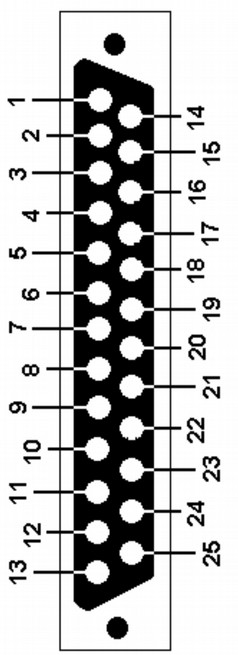
\includegraphics[height=4cm]{img/images-000.png}
  \end{minipage}
  \begin{minipage}[b]{0.5\textwidth}
    \centering
    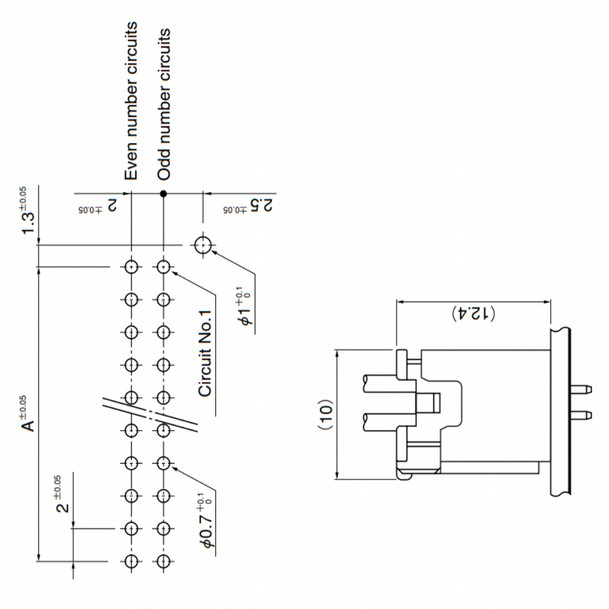
\includegraphics[height=6cm]{img/images-002.png}
  \end{minipage}
  \begin{minipage}[b]{0.2\textwidth}
    \centering
    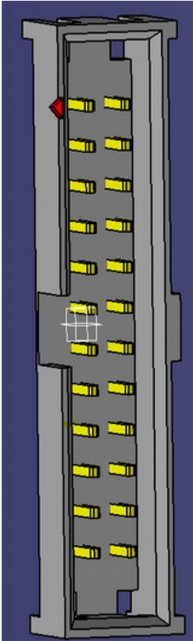
\includegraphics[height=4cm]{img/images-004.png}
  \end{minipage}
  \begin{minipage}[t]{0.2\textwidth}
    \centering
    \captionof{figure}{D-sub}
  \end{minipage}
  \begin{minipage}[t]{0.5\textwidth}
    \centering
    \captionof{figure}{JST B24B}
  \end{minipage}
  \begin{minipage}[t]{0.2\textwidth}
    \centering
    \captionof{figure}{SAMTEC\\STMM-112\\-01-S-D}
  \end{minipage}
\end{center}

\subsection{Front panel}
TODO

\subsection{Status LEDs}

Each channel has an LNA which is powered by a constant current driver that is inside the RD module.
The voltages of the two LNA constant-current drivers are polled every 5 seconds and the corresponding LEDs are updated accordingly. See section \ref{sec:ads1015} for more details about the conversion process.
When the voltage is between 2.2 (V) and 2.6 (V) the LNA is considered to be in good/normal operating conditions. When the voltage is either too high or too low this indicates a fault condition in the LNA or a connection issue between the RD module and the LNA. 

  \begin{tabular}{l|l}
    LED & description \\\hline
    constant off & RD not powered or not booted \\
    constant on  & RD powered up and LNA voltage inside expected range \\
    slow blink (once per second) & LNA voltage too high (no antenna connected) \\
    fast blink (3 times per second) & LNA voltage too low (antenna shorted)\\
  \end{tabular}
  
\begin{deprecation}
  Prior to firmware version 4 the behaviour was different:
  the LEDs are permanently on as soon as the RD is successfully booted.

  Physical modules prior to hardware version 3 do not have leds on the front panel.
\end{deprecation}

\begin{warning}
  It is planned but not yet implemented to make the LNA current configurable, in which case the thresholds will change as well.
\end{warning}


\section{Channel naming}
For historical reasons several conflicting naming conventions are used. The following table shows the matching between these conventions.

\begin{center}
\begin{tabular}{|l|l|l|l|l|l|l|}
  \hline
  RD channel &  Radio sensitivity & Antenna orientation & ADC channel & RD front panel & Offline channel \\
  \hline
  0 & from N/S & loop facing E/W & B & left & 1 \\
  1 & from E/W & loop facing N/S & A & right & 2 \\
  \hline
\end{tabular}
\end{center}
                                    

\section{Software interface}
The Auger \ac{RD} module has two separate interfaces.
One fast interface to capture radio traces, and one slower \ac{SPI} interface for housekeeping and metadata. 

\subsection{Radio data}
The Auger \ac{RD} module samples 12-bit data from 2 channels at 250 Msamples/s into a circular buffer.
It does so continuously until it sees a logic high on the trigger input.
When the trigger is received the \ac{RD} will continue to write a configurable number of post-trigger samples to the buffer.
The number of post-trigger samples can be configured using the housekeeping \ac{SPI} interface and defaults to 1024 at power-up.
The total buffer always contains 2048 samples and therefore the number of pre-trigger samples equals $2048-\text{\#(pre-trigger samples)}$.
See Section \ref{sec:trigger_offset} for details. 

When the post-trigger samples have been recorded, the transfer is automatically initiated.
Figures~\ref{fig:datatransferstart}~and~\ref{fig:datatransferfinish} show the data transfer protocol. 
The transfer is clocked from the RD at 60 MHz. The clock is held high outside the transmission windows.
\begin{warning}
  The 60 MHz speed is subject to change.
  Due to the distribution of events, it is suspected that a small reduction  in transfer time could benefit the number of recorded events greatly.
\end{warning}
The transmission starts with a preamble consisting of 4 rising clock edges.
After the preamble, the 2048 samples are transmitted. Data for the 2 channels is separately transmitted on the 2 data lines.
Each sample is shifted out, most significant bit first, followed by a parity bit (odd parity). Finally, 11 trailing clock cycles are transmitted.


\begin{center}
  \begin{minipage}[b]{\textwidth}
    \centering
    %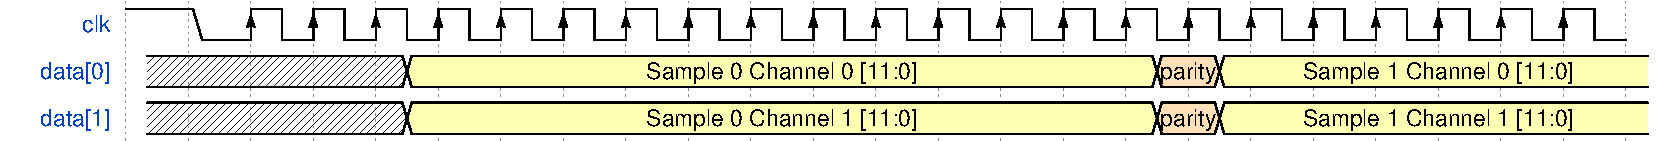
\includegraphics[width=\textwidth]{img/data-transfer-start.pdf}
    \begin{tikztimingtable}[timing/wscale=1.2]
      clk     & HHLCCCCCCCCCCCCCCCCCCCCCCCCCCCCCCCCCCCCCCCCCCCCCC \\ 
      data[0] & UUUUUUUUUUDDDDDDDDDDDDDDDDDDDDDDDD{Sample 0 Channel 0 [11:0]}DD{parity}DDDDDDDDDDDDD{Sample 1 Channel 0 [11:0]} \\
      data[1] & UUUUUUUUUUDDDDDDDDDDDDDDDDDDDDDDDD{Sample 0 Channel 1 [11:0]}DD{parity}DDDDDDDDDDDDD{Sample 1 Channel 1 [11:0]} \\
    \end{tikztimingtable}
    \captionof{figure}{Start of data transfer has 3 leading clock edges. Data is stable at rising edges. Parity bit follows data.}\label{fig:datatransferstart}
  \end{minipage}\vspace{\baselineskip}
  \begin{minipage}[b]{\textwidth}
    \centering
    %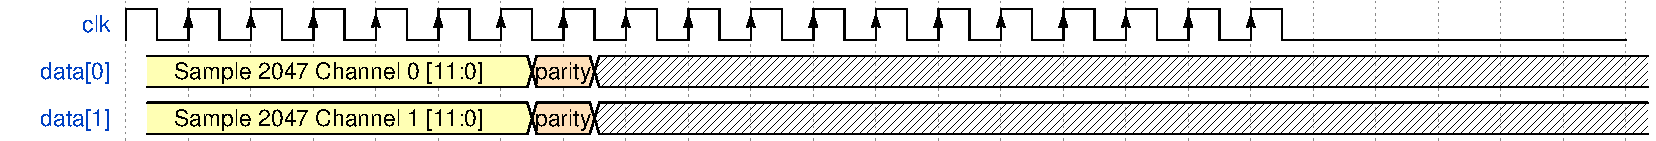
\includegraphics[width=\textwidth]{img/data-transfer-finish.pdf}
    \begin{tikztimingtable}[timing/wscale=1.2]
      clk     & CCCCCCCCCCCCCCCCCCCCCCCCCCCCCCCCCCCCCCCCHHHHHHH \\ 
      data[0] & DDDDDDDDDDDDDDDD{Sample 2047 Channel 0 [11:0]}DD{parity}UUUUUUUUUUUUUUUUUUUUUUUUUUUUU \\
      data[1] & DDDDDDDDDDDDDDDD{Sample 2047 Channel 1 [11:0]}DD{parity}UUUUUUUUUUUUUUUUUUUUUUUUUUUUU \\
    \end{tikztimingtable}
    
    \captionof{figure}{End of data transfer has 11 trailing rising edges.}\label{fig:datatransferfinish}
  \end{minipage}
\end{center}

There is negligeable delay between the registration of the last sample and the start of the transmission and between the end of the transmission and the registration of the first sample for the next trace.

During the transmission and during the recording of the pre-trigger samples the value of the trigger input is ignored.



\subsection{Jitter and latency}\label{sec:latency}
Data is transferred from an \ac{ADC} (ADS4229) to an \ac{FPGA} (Lattice ECP5 LFE5U-12F) over 12 LVDS pairs. The data transfer is \ac{DDR} which means that the even bits are transferred on the rising edges of the 250 MHz clock and the odd bits on the falling edges. 

There is at most one sample jitter on the data.

\begin{center}
  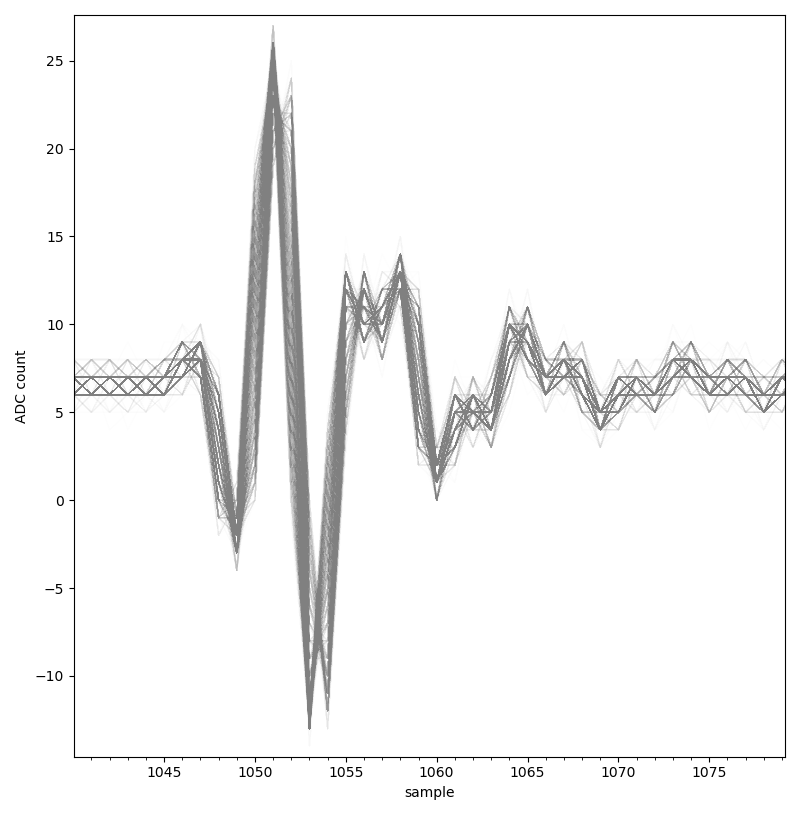
\includegraphics[width=0.8\textwidth]{img/trigger_jitter.png}
  \captionof{figure}{Trigger line fed back into data signal via an external probe. Note that the rising edge of the trigger is transformed into a wavelet by the analog filters on the RD. Two thousand traces are plotted over each other with high transparency.}\label{fig:trigger_jitter}
\end{center}

\begin{center}
  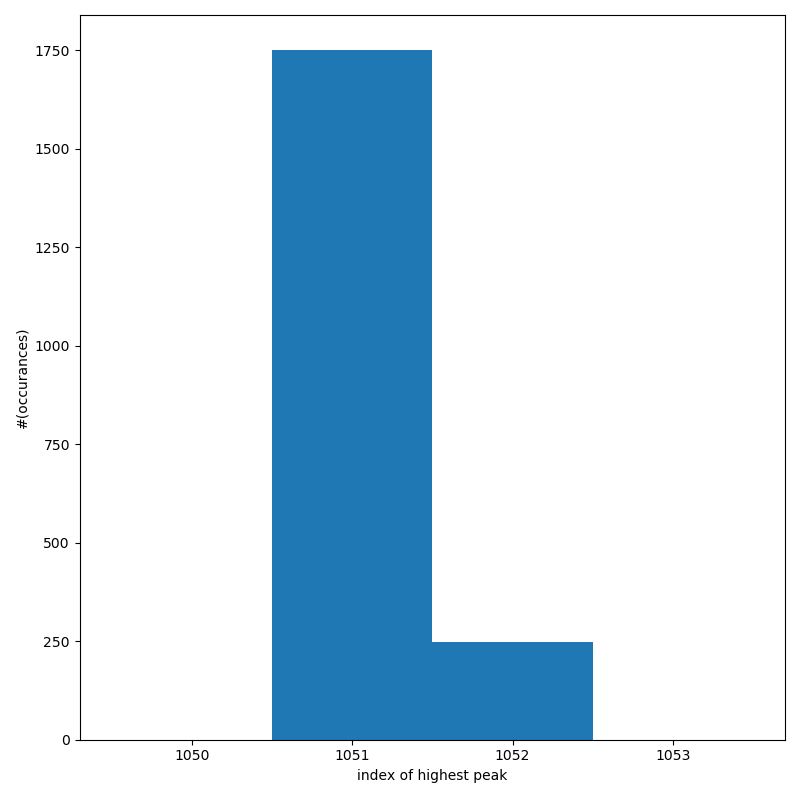
\includegraphics[width=0.8\textwidth]{img/trigger_hist.png}
  \captionof{figure}{Location of the highest peak in Figure~\ref{fig:trigger_jitter}.}\label{fig:trigger_location}
\end{center}

Using the trigger-offset feature of the \ac{SPI} housekeeping interface, the location of the data window relative to the trigger can be configured. By default the location is set to 1024. 
The \ac{ADC} is also subject to 16 clock cycles sampling latency.
In addition the clock propagation delay in the \ac{ADC} is typically 6.2 ns which is more than one sample at 250 MHz.
With the default trigger offset of 1024, all factors included, there are therefore 1041 samples before the trigger and 1007 samples after the trigger.

\begin{center}
  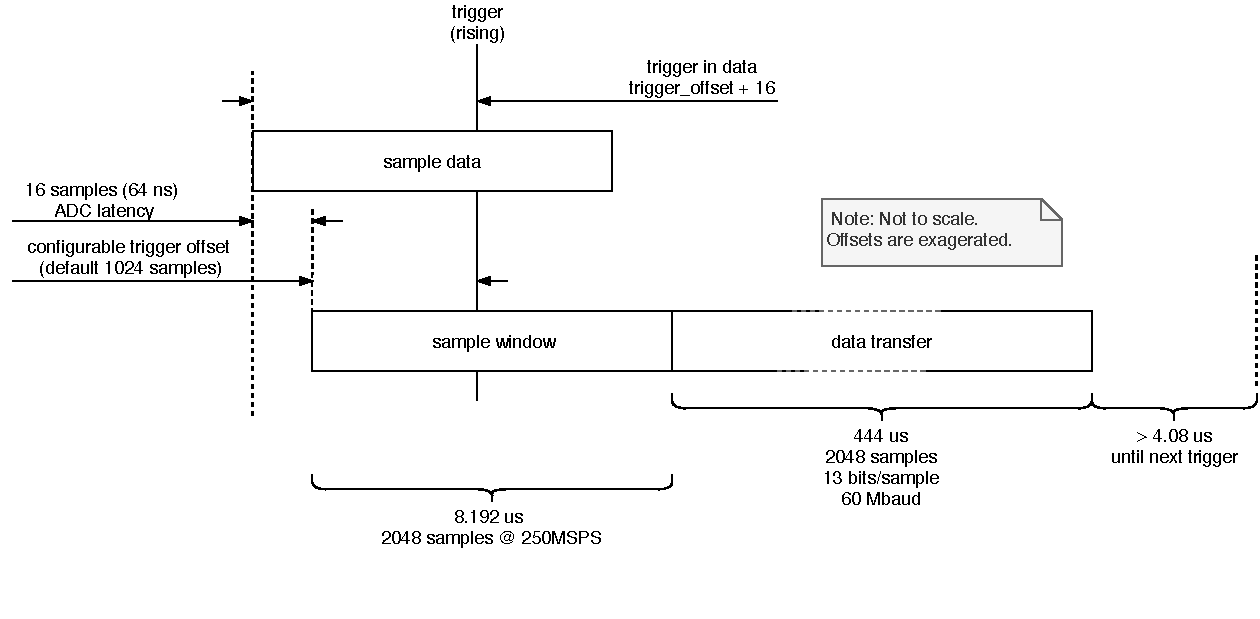
\includegraphics[width=\textwidth]{img/rd_timing_v2.pdf}
  \captionof{figure}{Timing of \ac{RD} capture.}\label{fig:rd_timing}
\end{center}

Figure~\ref{fig:rd_timing} summarizes the delays and time-offsets between trigger input and the data capture window.
Figures~\ref{fig:trigger_jitter} and \ref{fig:trigger_location} show experimentally determined trigger location in the trace window. Note that in this setup the trigger signal was picked up with an inductive probe and fed into the analog frontends of the RD board. This incurs additional delays which explains the (~20 ns) difference between the ideal trigger location (1041) and the start of the signal in Figure~\ref{fig:trigger_location} (1046). 

\begin{warning}
  In firmware versions prior to v4 the trigger was delayed by 4 samples due to clock synchonization. Including the 16 samples ADC latency, the trigger would fall on the 12th sample after the configured start offset instead of the 16th. There was also one additional sample jitter in the registration of the trigger which was removed in firmware version 4. 
\end{warning}


\subsection{\acs{SPI} housekeeping interface}

\subsubsection{General Architecture}
The \ac{SPI} interface exposes several features including: firmware updates, science \ac{ADC} re-configuration, \ac{GPIO} access, a temperature sensors, and readout of \ac{LNA}/bias status.
The latter provides operating voltages and currents independently on each channel.

All of the above features are handled by independent sub-systems that  are internally bridged by an \ac{SPI} demuxer. The first 8 bits of every \ac{SPI} transaction are captured by the demuxer. The remainder of the transaction is forwarded transparently to the sub-system in question.

An example program \texttt{rd\_housekeeping} is provided that exposes most of the available features. Refer to the source in the git repository\footnote{\url{https://github.com/auger-prime-sde/rd/tree/master/uub-linux-tools/rd_housekeeping}}.

\begin{center}
  \begin{tikztimingtable}
    clk                   & HH21{C} {[dotted]10{C}} 5{C}HH \\
    ce in                 & HH21{L} {[dotted]10{L}}5{L}HH \\
    mosi                  & UU16{D}{address, e.g. 0x06}5{D}[dotted]10{D}[solid]5{D}{forwarded data}UU \\    
    \ldots                & \\
    ce to sub-system 0x05 & 23{H} {[dotted]10{H}}7{H} \\
    ce to sub-system 0x06 & 18{H}5{L} {[dotted]10{L}} 5{L} 2{H} \\
    ce to sub-system 0x07 & 23{H} {[dotted]10{H}}7{H} \\
    \ldots                & \\
  \end{tikztimingtable}
  \captionof{figure}{\ac{SPI} demuxer example.}
\end{center}


\subsubsection{\acs{SPI} mode and speed}
The \ac{SPI} interface was tested upto 12 MHz. It is known that all sub-systems can also reach that speed.
The external interface operates with CPOL=1 and CPHA=1 (spi mode 3) at all times. The ADS4229 science adc operates in mode 2 but the responsible sub-system block handles the translation. All \ac{SPI} data is transferred \ac{MSB} first. 


\subsubsection{Housekeeping trigger}
The internal temperature, bias voltage and bias current sensors are automatically triggered every 5 seconds.
This updates the status leds as well as the internal registers that can be read out through the \ac{SPI} interface.

\subsubsection{\ac{GPIO} (address 0x01)}
Eight \ac{GPIO} pins are available on the \ac{RD} board. All pins are configured as outputs. The \ac{GPIO} sub-system allows writing to and reading from the output buffer. The \ac{GPIO} cannot be configured as input pins. Each transaction exists of a command byte, optionally followed by a data byte in case of a write command.

The supported commands are:
\begin{center}
  \begin{tabular}{|l|l|l|}
    \hline
    command & code & expects data \\
    \hline
    read & 0x00 & no \\
    write & 0x01 & yes \\
    set bits (gpio = gpio | data) & 0x02 & yes \\
    clear bits (gpio = gpio \& $\neg{}$ data) & 0x03 & yes \\
    reset to default (0xFF) & 0x04 & no \\
    \hline
  \end{tabular}
  \captionof{table}{\ac{GPIO} commands.}
\end{center}

\begin{center}
  \begin{tikztimingtable}
    clk  & HHCCCCCCCCCCCCCCCCCCCCCCCCCCCCCCCCCCCCCCCCCCCCCCCCHH \\
    ce   & HHLLLLLLLLLLLLLLLLLLLLLLLLLLLLLLLLLLLLLLLLLLLLLLLLHH \\
    mosi & UUDDDDDDDDDDDDDDDD{0x01 (select \ac{GPIO})}DDDDDDDDDDDDDDDD{0x00 (\ac{GPIO} read)}UUUUUUUUUUUUUUUUUU \\
    miso & UUUUUUUUUUUUUUUUUUUUUUUUUUUUUUUUUUDDDDDDDDDDDDDDDD{0x42 (for example)}UU \\
  \end{tikztimingtable}
  \vspace{\baselineskip}\\
  \begin{tikztimingtable}
    clk  & HHCCCCCCCCCCCCCCCCCCCCCCCCCCCCCCCCCCCCCCCCCCCCCCCCHH \\
    ce   & HHLLLLLLLLLLLLLLLLLLLLLLLLLLLLLLLLLLLLLLLLLLLLLLLLHH \\
    mosi & UUDDDDDDDDDDDDDDDD{0x01 (select \ac{GPIO})}DDDDDDDDDDDDDDDD{0x01 (\ac{GPIO} write)}DDDDDDDDDDDDDDDD{0x00 (for example)}UU \\
    miso & UUUUUUUUUUUUUUUUUUUUUUUUUUUUUUUUUUDDDDDDDDDDDDDDDD{0x42 (old data)}UU \\
  \end{tikztimingtable}
  \captionof{figure}{Example \ac{GPIO} read and write. The output register contains the data 0x42 and is written to 0x00.}
\end{center}


\subsubsection{Program flash pass-through (address 0x02)}
Transactions to address 0x02 are forwarded transparently to the \ac{SPI} flash chip.
This flash chip uses a standard JEDEC interface.
Refer to the SST26VF032B documentation for details.

\begin{center}
  \begin{tikztimingtable}[timing/wscale=0.6]
    clk      & HHCCCCCCCCCCCCCCCCCCCCCCCCCCCCCCCCCCCCCCCCCCCCCCCCCCCCCCCCCCCCCCCCCCCCCCCCCCCCCCCCHH \\
    uub ce   & HHLLLLLLLLLLLLLLLLLLLLLLLLLLLLLLLLLLLLLLLLLLLLLLLLLLLLLLLLLLLLLLLLLLLLLLLLLLLLLLLLHH \\
    flash ce & HHHHHHHHHHHHHHHHHHLLLLLLLLLLLLLLLLLLLLLLLLLLLLLLLLLLLLLLLLLLLLLLLLLLLLLLLLLLLLLLLLHH \\
    mosi     & UUDDDDDDDDDDDDDDDD{0x02 (select \ac{SPI} flash)}DDDDDDDDDDDDDDDD{0x9F (read id)}UUUUUUUUUUUUUUUUUUUUUUUUUUUUUUUUUUUUUUUUUUUUUUUUUU \\
    miso     & UUUUUUUUUUUUUUUUUUUUUUUUUUUUUUUUUUDDDDDDDDDDDDDDDD{0xBF}DDDDDDDDDDDDDDDD{0x26}DDDDDDDDDDDDDDDD{0x42}UU\\
  \end{tikztimingtable}
  \captionof{figure}{Example SST26VF032B JEDEC-ID readout.}
\end{center}

The flash chip contains the FPGA user code that is loaded upon power-on.
A Primary and a Golden Pattern are present. If the checksum of the Primary Pattern fails the address in the JUMP command section is used to locate the Golden Pattern.

\begin{center}
  \begin{tabular}{llll}
    Start & End & Contents & Description\\\hline
    0x00 00 00 & 0x0A FF FF & Primary Pattern & Contains the user-code for the FPGA\\
    0x0B 00 00 & 0x15 FF FF & Golden Pattern & Fallback code for the FPGA\\
    0x16 00 00 & 0x3F F0 00 & Calibration file & Ascii encoded calibraton data\\
    0x3F FF 00 & 0x3F FF FF & JUMP command & Start address of the Golden Pattern\\
  \end{tabular}
  \captionof{table}{Flash layout.}
\end{center}

If the Primary Pattern does not pass a checksum validation (e.g. after an interrupted write) the Golden Pattern is loaded instead. The Golden Pattern implements a version of the firmware that contains nothing else except SPI access to the program flash such that the incomplete image may be restored.
Refer to the Lattice Dual Boot and Multiple Boot Features Techical Note (TN1216) for details about the dual boot procedure\footnote{\url{https://www.latticesemi.com/-/media/LatticeSemi/Documents/ApplicationNotes/AD/DualandMulitpleBootFeature.ashx}}.

Neither the JUMP command not the Golden Pattern should be overwritten.
An example program \texttt{rd\_flash} is provided which performs safe read and write methods to dump and write the Primary Pattern from a bit-file.
Refer to the source in the git repository\footnote{\url{https://github.com/auger-prime-sde/rd/tree/master/uub-linux-tools/rd_flash}}.

Note that a small gap is left unused between the calibration data and the jump command. This is to ensure that the jump command does not share eraseable sectors with the userdata. I.e., writing the last page of the user data does not require clearing (and therefore re-writing) the jump command.

The provided \texttt{rd\_flash} tool will prohibit writes over the golden images, the jump command, or the calibration file. Note that the SPI flash interface itself provides no such protection. It is possible to brick the RD module if the sectors are erased.

\begin{warning}
  The first 6 RD module deployed in November 2019 are not equiped with a Golden Pattern or calibration section.
\end{warning}



\subsubsection{Science ADC configuration SPI pass-through (address 0x03)}
The science \ac{ADC} has a \ac{SPI} configuration interface. The ADS4229 expects \ac{SPI} mode 2 (cpol=1, cpha=0) but also works in \ac{SPI} mode 1 (cpol=0, cpha=1) which is achieved by inverting the clock signal from the \ac{UUB} interface.

\begin{center}
  \begin{tikztimingtable}[timing/wscale=1]
    uub spi clk & HHCCCCCCCCCCCCCCCCCCCCCCCCCCCCCCCCCCCCCCCCCCCCCCCCHH \\
    uub spi ce  & HHLLLLLLLLLLLLLLLLLLLLLLLLLLLLLLLLLLLLLLLLLLLLLLLLHH \\
    mosi        & UUDDDDDDDDDDDDDDDD{0x03 (select ADS4229 adc)}DDDDDDDDDDDDDDDD{0x25 (gain register)}DDDDDDDDDDDDDDDD{0x40 gain setting}UU \\
    adc spi ce  & HHHHHHHHHHHHHHHHHHLLLLLLLLLLLLLLLLLLLLLLLLLLLLLLLLHH \\
    adc spi clk & LLLLLLLLLLLLLLLLLLCCCCCCCCCCCCCCCCCCCCCCCCCCCCCCCCLL \\
  \end{tikztimingtable}
  \captionof{figure}{Example ADS4229 transaction. This sets the channel A gain (config register address 0x25) to 2dB.}
\end{center}

Refer to the ADS4229 datasheet \footnote{\url{http://www.ti.com/lit/ds/symlink/ads4229.pdf}} for details on the available registers in the configuration interface.


\subsubsection{ADS1015 current and voltage sensors (address 0x04)}\label{sec:ads1015}
The ADS1015 is a four port \ac{I2C} \ac{ADC} which is wired to measure the voltage and the current on both \ac{LNA} channels. This can be used to determine if the \ac{LNA} is properly connected and working as expected.

\begin{deprecation}
    This behaviour is not yet implemented in firmware version 3. In this version a conversion is triggered after the sample buffer write cycle is completed. 
\end{deprecation}

Periodically (every 5 seconds) the internal controller for this \ac{I2C} chip will execute a fixed sequence of \ac{I2C} commands and store the conversion result in a register. The register can be read via \ac{SPI} and contains eight bytes:

\begin{center}
  \begin{tabular}{|l|l|}
    \hline
    Register address & contents \\
    \hline
    0x00 & bits [11:4] of \acs{ADC} channel 0 (N/S bias current)\\
    0x01 & bits [3:0]  of \acs{ADC} channel 0, followed by four zeroes\\
    0x02 & bits [11:4] of \acs{ADC} channel 1 (N/S bias voltage)\\
    0x03 & bits [3:0]  of \acs{ADC} channel 1, followed by four zeroes \\
    0x04 & bits [11:4] of \acs{ADC} channel 2 (E/W bias current)\\
    0x05 & bits [3:0]  of \acs{ADC} channel 2, followed by four zeroes \\
    0x06 & bits [11:4] of \acs{ADC} channel 3 (E/W bias voltage)\\
    0x07 & bits [3:0]  of \acs{ADC} channel 3, followed by four zeroes \\
    \hline
  \end{tabular}
  \captionof{table}{ADS1015 register layout.}
\end{center}

The ADS1015 has a \ac{PGA}. All conversions are made with the $FSR=\pm4.096 V$ setting. I.e. $MSB = 2 mV$.
Note that the bias voltage is measured over a 1:1 voltage divider so the actual bias voltage is twice that of the measured inputs.
The bias currents are measured with a 200 V/V current sensing amplifier over a $0.2\Omega$ current sensing resistor. I.e., the bias current is $0.025 * V_{\text{ADC voltage}}$.

To read a byte from the register, write the address of that register and read the data on the next byte. The next address can already be written during the read and therefore the whole register can efficiently be retrieved in a 10-byte transaction (including the sub-system address byte). 
If the readout overlaps with a new measurement the readout is guaranteed to return consistent sample values.


\begin{center}
  \begin{tikztimingtable}[timing/wscale=0.8]
    clk  & HHCCCCCCCCCCCCCCCCCCCCCCCCCCCCCCCCCCCCCCCCCCCCCCCCCCCCCCCCCCCCCCCCHH \\
    ce   & HHLLLLLLLLLLLLLLLLLLLLLLLLLLLLLLLLLLLLLLLLLLLLLLLLLLLLLLLLLLLLLLLLHH \\
    mosi & UUDDDDDDDDDDDDDDDD{0x04 (select ADS1015)}DDDDDDDDDDDDDDDD{0x04}DDDDDDDDDDDDDDDD{0x05}UUUUUUUUUUUUUUUUUU \\
    miso & UUUUUUUUUUUUUUUUUUUUUUUUUUUUUUUUUUDDDDDDDDDDDDDDDD{$I_{E/W}[11:4]$}DDDDDDDD{$I_{E/W}[3:0]$}DDDDDDDD{0000}UU \\
  \end{tikztimingtable}
  \captionof{figure}{Example ADS1015 register readout for the E/W \ac{LNA} bias current.}
\end{center}


\subsubsection{SI7060 temperature sensor (address 0x05)}
The Si7060 is an \ac{I2C} temperature sensor which measures the temperature inside the \ac{RD} enclosure.

\begin{warning}
  This behaviour is not yet implemented in firmware version 3. In this version a conversion is triggered after the sample buffer write cycle is completed. 
\end{warning}

Periodically (every 5 seconds), the controller for this \ac{I2C} chip will execute a fixed sequence of \ac{I2C} commands and stores the conversion result in a register. The register can be read via \ac{SPI} and contains two bytes:

\begin{center}
  \begin{tabular}{|l|l|}
    \hline
    Register address & contents \\
    \hline
    0x00 & Dspsigm of Si7060 (one status bit and data bits [14:8])\\
    0x01 & Dspsigl of Si7060 (data bits [7:0])\\
    \hline
  \end{tabular}
  \captionof{table}{Si7060 register layout.}
\end{center}



The raw 15-bit data is calculated as:
$$
D =  \text{Dspsigm}[6:0] < < 8 + \text{Dspsigl}[7:0]
$$

The temperature can be calculated as follows:
$$
T (^\circ{}C) = 55 + (D - 16384) / 160
$$



To read a byte from the register simply write the address of that register and read the data on the next byte. The next address can already be written during the read and therefore the whole register can efficiently be read in one 4-bute transaction (including the sub-system address byte).
If the readout overlaps with a new measurement the readout is guaranteed to return consistent sample values.

\begin{center}
  \begin{tikztimingtable}[timing/wscale=0.8]
    clk  & HHCCCCCCCCCCCCCCCCCCCCCCCCCCCCCCCCCCCCCCCCCCCCCCCCCCCCCCCCCCCCCCCCHH \\
    ce   & HHLLLLLLLLLLLLLLLLLLLLLLLLLLLLLLLLLLLLLLLLLLLLLLLLLLLLLLLLLLLLLLLLHH \\
    mosi & UUDDDDDDDDDDDDDDDD{0x05 (select Si7060)}DDDDDDDDDDDDDDDD{0x00}DDDDDDDDDDDDDDDD{0x01}UUUUUUUUUUUUUUUUUU \\
    miso & UUUUUUUUUUUUUUUUUUUUUUUUUUUUUUUUUUDDDDDDDDDDDDDDDD{Dspsigm}DDDDDDDDDDDDDDDD{Dspsigl}UU \\
  \end{tikztimingtable}
  \captionof{figure}{Example Si7060 temperature readout.}
\end{center}







\subsubsection{Version info (address 0x07)}
This sub-system will always return a 1-byte version code.
The currently known version codes are:
\begin{center}
  \begin{tabular}{|l|l|}
    \hline
    Code & Description \\
    \hline
    0x00 & legacy (version info not implemented) \\
    0x01, 0x02 & used during development \\
    0x03 & version shipped with \ac{RD} v3 units for the Malargue engineering array in November 2019\\
    0xFE & fallback image used in the golden pattern\\
    0xFF & may indicate SPI communication error on the UUB\\
    \hline
  \end{tabular}
\end{center}

\begin{center}
  \begin{tikztimingtable}[timing/wscale=0.8]
    clk  & HH32{C}HH \\
    ce   & HH32{L}HH \\
    mosi & UU16{D}{0x07 (select version)}16{U}UU \\
    miso & UU16{U}16{D}{0x03 (version code)}UU \\
  \end{tikztimingtable}
  \captionof{figure}{Example version read.}
\end{center}






\subsubsection{Trigger-offset configuration(address 0x08)}\label{sec:trigger_offset}
The position of the trigger within the data window can be configured.
This trigger-offset is set to 1024 (mid window) on power up but can be changed using this interface.
The value is set by writing two bytes to this sub-system. Only the lower 11 bits are used. The upper 5 bits are ignored.
The written number represents the position in the data trace where the trigger will be located. Note that the actual trigger appears at a slightly different position due to latency in the \ac{ADC} and in the \ac{RD}. Refer to Figure~\ref{fig:rd_timing} for details.
\begin{center}
  \begin{tikztimingtable}[timing/wscale=1]
    clk  & HHCCCCCCCCCCCCCCCCCCCCCCCCCCCCCCCCCCCCCCCCCCCCCCCCHH \\
    ce   & HHLLLLLLLLLLLLLLLLLLLLLLLLLLLLLLLLLLLLLLLLLLLLLLLLHH \\
    mosi & UUDDDDDDDDDDDDDDDD{0x08 (select offset reg)}UUUUUUUUUUDDDDDD{offset[11:8]}DDDDDDDDDDDDDDDD{offset[7:0]}UU \\
  \end{tikztimingtable}
  \captionof{figure}{Example start-offset setting transaction.}
\end{center}

Values of 0, 1, 2047 and 2048 are not permissible.
\begin{warning}
  In the next firmware update this constraint will be dropped.
\end{warning}


\subsection{Do not use (address 0x09)}
Used internally for debugging. Do not use.

\subsection{Enable/disable bias (address 0x0A)}
Power to the antenna can be disabled. It is on by default on boot and changes do not persist over power cycles.
The digital interface is identical to the GPIO except that the output of the register is not available as pins on the digitizer board but used to control the bias circuit:
\begin{center}
  \begin{tabular}{|l|l|l|l|l|l|l|l|l|}
    \hline
    Bit & 7 & 6 & 5 & 4 & 3 & 2 & 1 & 0 \\
    \hline
    Function & N/A & N/A & N/A & N/A & N/A & N/A & EW bias & NS bias\\
    \hline
  \end{tabular}
\end{center}
  
\subsection{Raw data access (address 0x0B)}
Raw data can be captured completely independent of the trigger and fast readout.
This also allows access to longer consecutive traces than the normal data pipeline.
Upto 8192 samples can be retrieved via this interface.
Samples are continuously stored in a circular buffer. When a transaction to address 0x0B is started the write process is temporarily paused and the data is returned.
It is not mandatory to read the whole buffer. E.g., it is allowed to read 2048 samples and then release the CE line. This will cause the write process to resume.
There are no precautions that inhibit reads while the buffer was not fully overwritten. There is no parity information in this buffer.
There is a 13th bit with each sample that represents the value of the trigger input at that sample. For the EW channel this is sampled at the falling edge of the sample clock. I.e. there is 500 MSPS information on the trigger input line. This is in the last/highest bit of each sample.

The returned data is tightly packed (i.e., no aligned to bytes). Bits in the sample are transferred MSB first.
The oldest sample is transmitted first and the newest last.
The samples from the NS and EW channel are interleaved, starting with a NS sample, followed by the corresponding EW sample.

\begin{warning}
  This sub-system was used for debugging and may or may not be included in releases.
  In some cases the available memory may be reduced to 2048 or 4096 samples if other modules require more memory.
\end{warning}

\subsection{Boot time and boot sequence}
After power is applied the \ac{FPGA} loads its configuration from the SST26VF032B \ac{SPI} flash.
As soon as the user code is running the \ac{RD} executes a hard-coded initialization sequence on the \ac{SPI} interface, as if the \ac{UUB} had sent the following commands:

\begin{center}
  \begin{tabular}{|l|l|}
    \hline
    \acs{SPI} commands & Description \\
    \hline
    \texttt{0x03 0x00 0x02} & ADS4229 software reset \\
    \texttt{0x03 0x29 0x00} & re-assert default configuration \\
    \texttt{0x03 0x41 0x00} & re-assert default configuration \\
    \texttt{0x03 0x03 0x03} & enable high-performance mode \\
    \texttt{0x03 0xF2 0x00} & disable low speed mode (already off by default)\\
    \texttt{0x03 0xEF 0x00} & disable low speed mode (already off by default)\\
    \texttt{0x03 0x41 0x00} & cmos mode off (already off by default)\\
    \texttt{0x03 0x02 0x40} & enable high performance mode \\
    \texttt{0x03 0xD5 0x18} & enable high performance mode \\
    \texttt{0x03 0xD7 0x0C} & enable high performance mode \\
    \texttt{0x03 0xDB 0x20} & enable high performance mode \\
    \texttt{0x08 0x04 0x00} & set trigger-offset to 1024 \\
    \hline
  \end{tabular}
  \captionof{table}{\ac{RD} initialization sequence. }
  
\end{center}

This initialization sequences takes approximately 170 us. During this time the \ac{SPI} lines from the \ac{UUB} are inhibited and the MISO line will remain silent.



\end{document}